\documentclass[a4paper]{article}
\usepackage{a4wide}
\usepackage{amsmath}
\usepackage{amsfonts}
  \DeclareMathOperator*{\argmax}{arg\,max}
  \newcommand{\ex}[1]{{\mathbb E}\left[ #1 \right]}
  \newcommand\norm[1]{\left\lVert#1\right\rVert}
\usepackage{booktabs}
\usepackage{csquotes}
\usepackage{upquote}
\usepackage{float}
\usepackage{graphicx}
\usepackage{enumerate}
\usepackage{subcaption}
\usepackage{xcolor}


\title{Pattern and Speech Recognition WS2015-16 \\ Exercise 5}
\author{Atanas Poibrenski(2554135), Marimuthu Kalimuthu(2557695), Furkat Kochkarov(2557017)}

\begin{document}

\maketitle 
\begin{center}
	\textbf{Gaussian Mixture Models} 
\end{center}

\section*{1 Data Preparation}

\begin{enumerate}
	\item[ \textbf{Ex-1} ] Done.
	\item[ \textbf{Ex-2} ] Loaded data into 677970x50 matrix and removed the first column(which is the useless dimension). (See `data\_preparation.m')
	\item[ \textbf{Ex-3} ] We used \textit{pca} function of matlab and selected the first dimension of the projected data. (See data\_preparation.m)
	\item[ \textbf{Ex-4} ] We plot the distribution using histogram with 200 bins to get a clear idea of the distribution of the data. The cluster size is 5 because the histogram resembles five separate groups of points.

	\begin{figure}[H]
		\begin{center}
			\includegraphics[width=1.2\textwidth]{hist.eps}
			\caption{Data distribution - histogram with 200 bins}\label{fig:histdist}
		\end{center}
	\end{figure}

\end{enumerate}


\section*{2 Clustering uing K-Means}
\subsection*{2.1 Cluster Association}
\begin{enumerate}
	\item[\textbf{Ex-5}] See `rmse.m'
	\item[\textbf{Ex-6}] See `associate.m'
\end{enumerate}

\subsection*{2.2 Compute Means}
\begin{enumerate}	
	\item[ \textbf{Ex-7} ] It should be (k x N) since we want to compute \textbf{k} amount of \textit{means}  and each \textit{mean} will be of the dimension of the data which is \textbf{N}.
	\item[ \textbf{Ex-8} ] See `compute\_means.m'
\end{enumerate}


\subsection*{2.3 Initialization}
\begin{enumerate}	
	\item[ \textbf{Ex-9} ] 	We set the initial \textbf{k} means as random \textbf{k} points from the data. This performs better than random initialization. When we used random initializations, some clusters remain unassigned to data points which requires additional steps to deal with.
\end{enumerate}

\subsection*{2.4 K-Means}
\begin{enumerate}	
	\item[ \textbf{Ex-10} ] See `kmeans\_.m'
	\item[ \textbf{Ex-11} ] cluster means plot
	
	\begin{figure}[H]
		\begin{center}
			\includegraphics[width=1.1\textwidth]{clusters_means.eps}
			\caption{means of all clusters}\label{fig:clustermean}
		\end{center}
	\end{figure}
	
\end{enumerate}


\section*{3 GMM initialization}
\begin{enumerate}
	\item[\textbf{Ex-12}]
	
	Means: [-0.0086	-3.6375	-8.2074 9.2524 4.0791 ]
	
	Covs:  [0.2669 1.5800 0.9207 0.8581 1.3088]
	
	Weights: [ 0.8650	0.0502	0.0209	0.0198	0.0438 ]
	
	(Also see `gmm\_init.m')
	
	\item[\textbf{Ex-13}] We have defined 5 Gaussians with separate weights which is the definition of Gaussian Mixture Model. Instead of using EM algorithm, we used the final clusters from  `kmeans' algorithm.
	\item[\textbf{Ex-14}](\textbf{Bonus}) GMM-Plot
	\begin{figure}[H]
		\begin{center}
			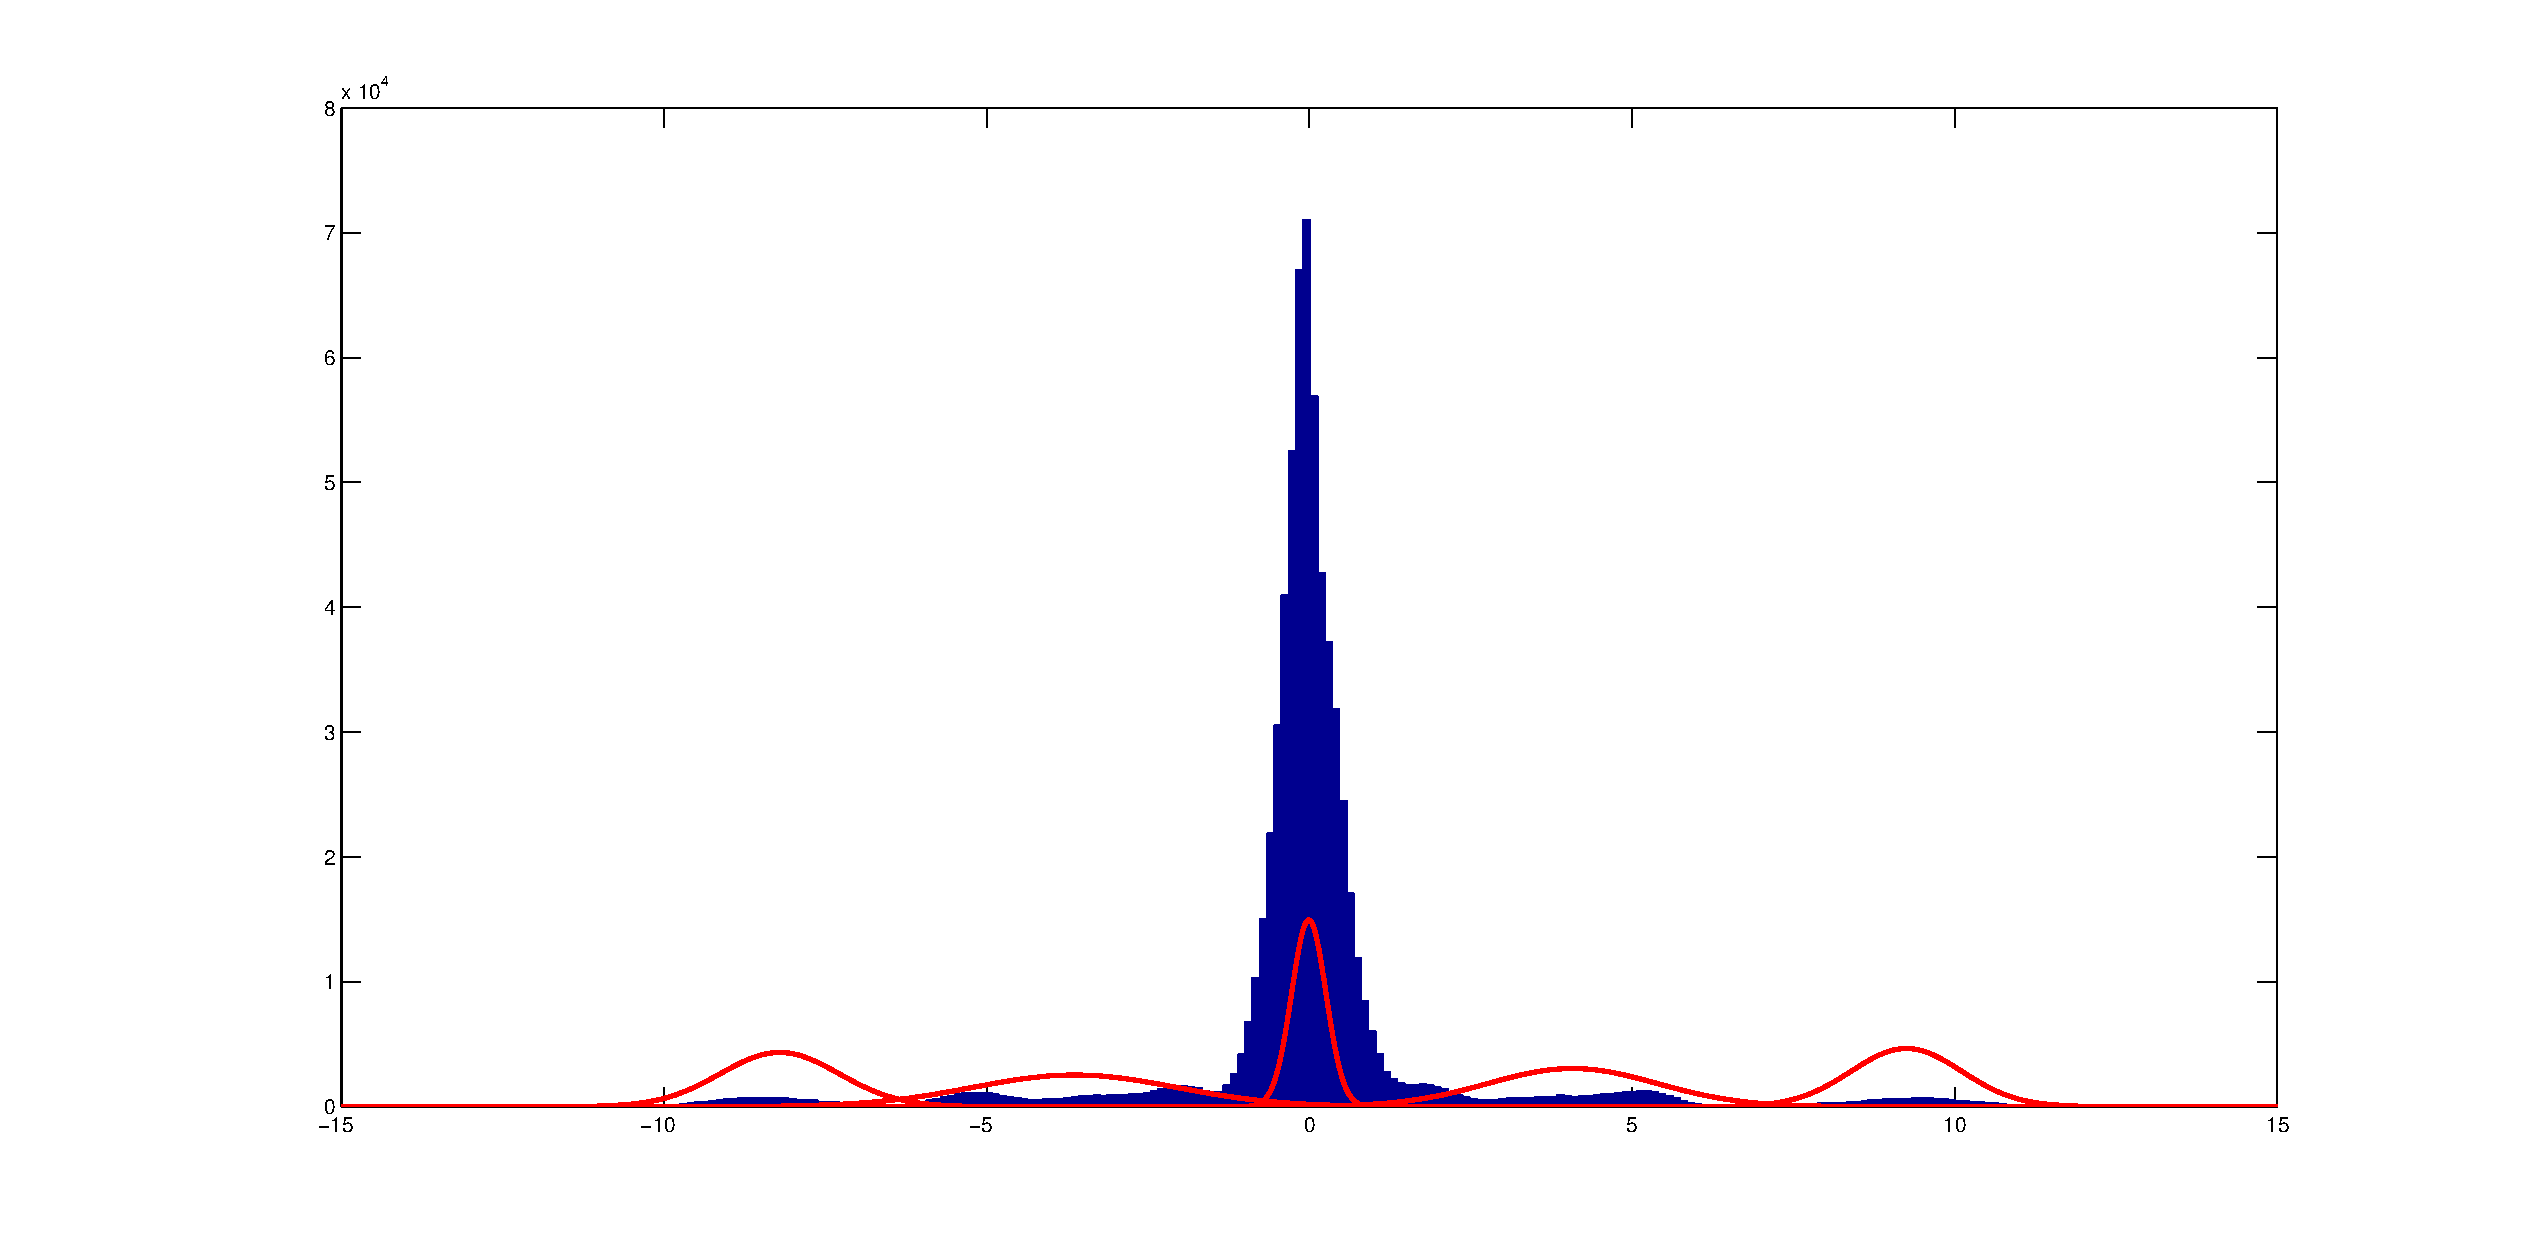
\includegraphics[width=1.1\textwidth]{gmm_hist.eps}
			\caption{Overlay of histogram and Gaussians}\label{fig:gmmhist}
		\end{center}
	\end{figure}	
\end{enumerate}


\section*{4 Application to the real data set}
\begin{enumerate}
	\item[\textbf{Ex-15}] Done. See all code!
\end{enumerate}


\end{document}
